\documentclass[paper=a4, fontsize=11pt]{scrartcl}
\usepackage[T1]{fontenc}
\usepackage{fourier}

\usepackage[english]{babel}															% English language/hyphenation
\usepackage[protrusion=true,expansion=true]{microtype}	
\usepackage{amsmath,amsfonts,amsthm} % Math packages
\usepackage[pdftex]{graphicx}	
\usepackage{url}
\usepackage{listings}
\usepackage{xcolor}
\usepackage{physics}

\definecolor{codegreen}{rgb}{0,0.6,0}
\definecolor{codegray}{rgb}{0.5,0.5,0.5}
\definecolor{codepurple}{rgb}{0.58,0,0.82}
\definecolor{backcolour}{rgb}{0.95,0.95,0.92}

\lstdefinestyle{mystyle}{
    backgroundcolor=\color{backcolour},   
    commentstyle=\color{codegreen},
    keywordstyle=\color{magenta},
    numberstyle=\tiny\color{codegray},
    stringstyle=\color{codepurple},
    basicstyle=\ttfamily\footnotesize,
    breakatwhitespace=false,         
    breaklines=true,                 
    captionpos=b,                    
    keepspaces=true,                 
    numbers=left,                    
    numbersep=5pt,                  
    showspaces=false,                
    showstringspaces=false,
    showtabs=false,                  
    tabsize=2
}

\lstset{style=mystyle}


%%% Custom sectioning
\usepackage{sectsty}
\allsectionsfont{\centering \normalfont\scshape}


%%% Custom headers/footers (fancyhdr package)
\usepackage{fancyhdr}
\pagestyle{fancyplain}
\fancyhead{}											% No page header
\fancyfoot[L]{}											% Empty 
\fancyfoot[C]{}											% Empty
\fancyfoot[R]{\thepage}									% Pagenumbering
\renewcommand{\headrulewidth}{0pt}			% Remove header underlines
\renewcommand{\footrulewidth}{0pt}				% Remove footer underlines
\setlength{\headheight}{13.6pt}


%%% Equation and float numbering
\numberwithin{equation}{section}		% Equationnumbering: section.eq#
\numberwithin{figure}{section}			% Figurenumbering: section.fig#
\numberwithin{table}{section}				% Tablenumbering: section.tab#


%%% Maketitle metadata
\newcommand{\horrule}[1]{\rule{\linewidth}{#1}} 	% Horizontal rule

\title{
		%\vspace{-1in} 	
		\usefont{OT1}{bch}{b}{n}
		\normalfont \normalsize \textsc{Quantum Mechanics I} \\ [25pt]
		\horrule{0.5pt} \\[0.4cm]
		\huge Project 1 \\
		\horrule{2pt} \\[0.5cm]
}
\author{
		\normalfont 								\normalsize
        Clayton Seitz\\[-3pt]		\normalsize
        \today
}
\date{}


%%% Begin document
\begin{document}
\maketitle

\section{Part I}


Here, we are trying to solve for the solutions to Schrodinger's eigenvalue equation:

\begin{equation*}
\hat{H}_{0}\phi_{n} = \epsilon_{n}\phi_{n}
\end{equation*}

By discretizing $\phi_{n}$, each $\phi_{n}$ becomes a finite dimensional vector and we can write $\hat{H}$ explicitly as a matrix. That matrix satisfies

\begin{equation*}
\sum_{j}\bra{i}\hat{H}_{0}\ket{j}\vec{\phi}_{n,j} = \epsilon_{n}\vec{\phi}_{n}
\end{equation*}

wheree $\bra{i}\hat{H}_{0}\ket{j}$ is the matrix element $[H_{0}]_{ij}$. It was shown the Schrodingers wave equation could be expressed in discrete form, as

\begin{equation*}
-t(\phi_{n,i+1} + \phi_{n,i-1}) + (2t+V_{i})\phi_{n,i} = \epsilon_{n}\phi_{n,i}
\end{equation*}

which gives us a relationship between $\phi_{n,i}$ and the neighboring elements $\phi_{n,i-1}$ and $\phi_{n,i+1}$. The eigenvalues equation can then be written as a matrix multiplication

\begin{equation*}
\hat{H}_{0}\phi_{n} = \begin{pmatrix}
2t + V_{1} & -t & 0 & \hdots\\
-t & 2t + V_{2} & -t& \hdots\\
0 & -t & 2t + V_{3}& \hdots\\
\vdots & \vdots & \vdots & \ddots
\end{pmatrix}
\begin{pmatrix}
\phi_{n,1}\\
\phi_{n,2}\\
\phi_{n,3}\\
\vdots
\end{pmatrix}
\end{equation*}

To show that the eigenvectors form an orthonormal set, We can define a matrix $T$ such that each column of $T$ is one eigenvector of $\hat{H}_{0}$. If the eigenvectors are indeed orthonormal, then

\begin{equation*}
T^{T}T = I_{N\times N}
\end{equation*}

\begin{figure}
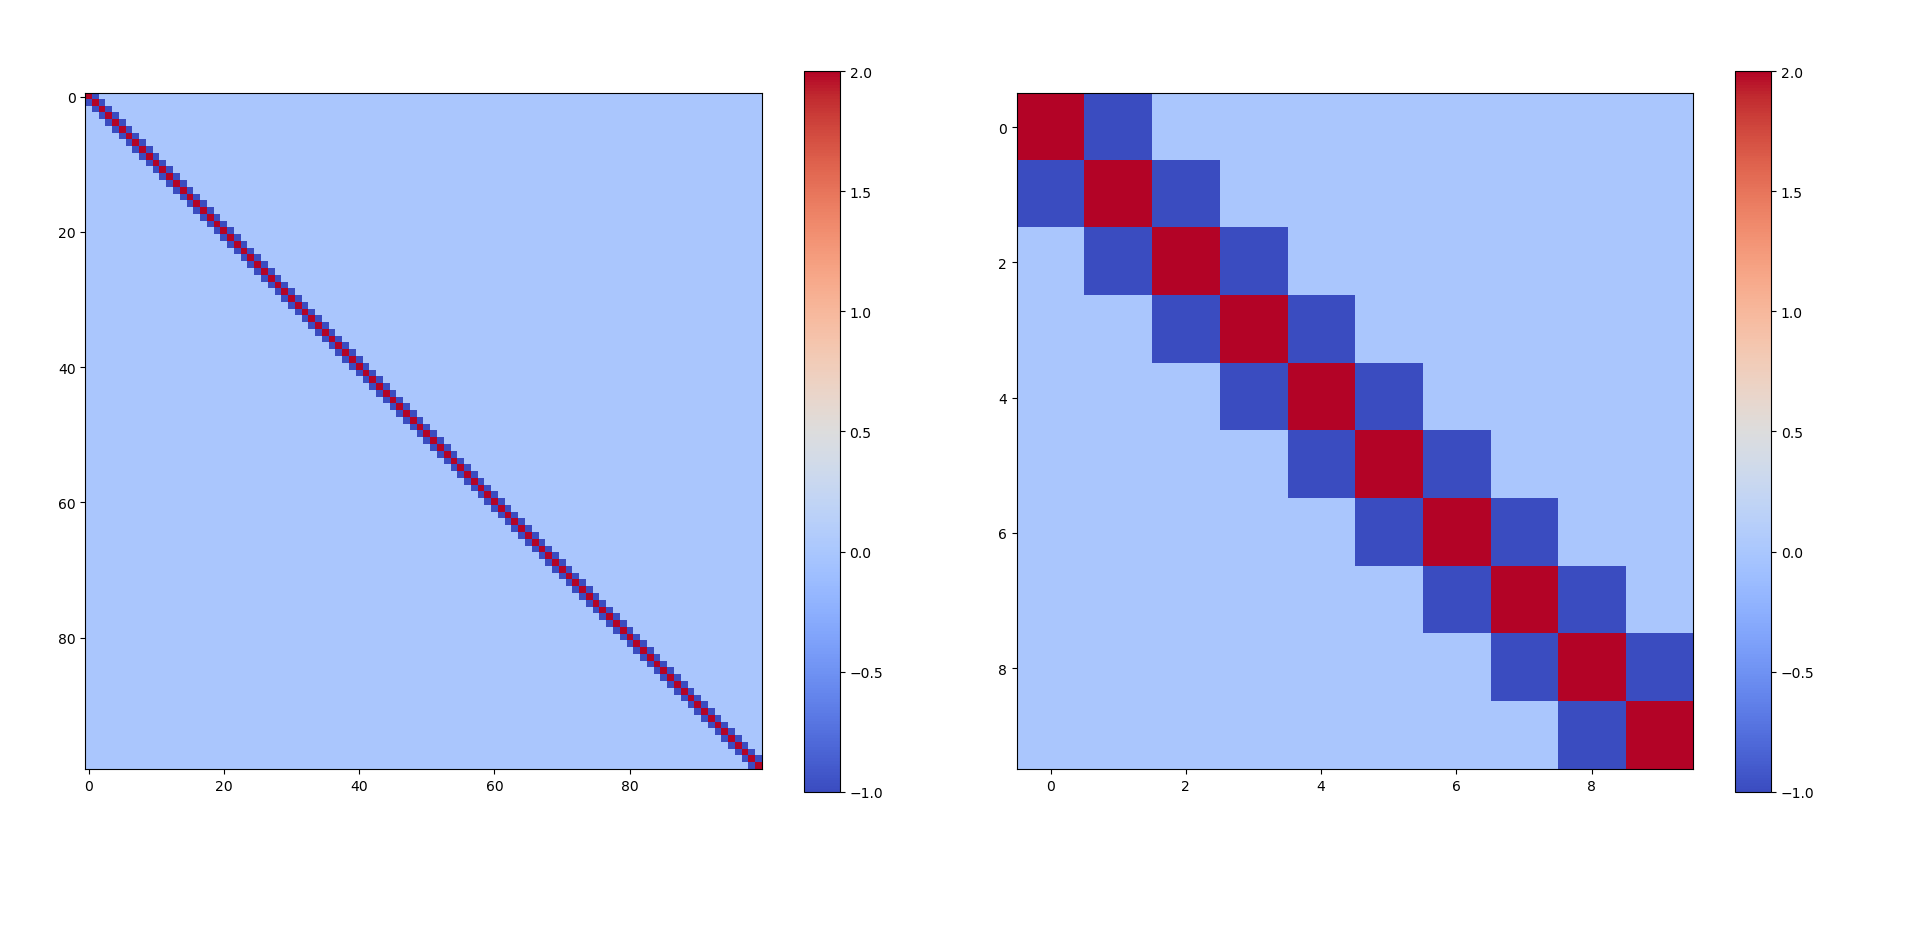
\includegraphics[width=14cm]{p1_1.png}
\caption{}
\end{figure}

\begin{figure}
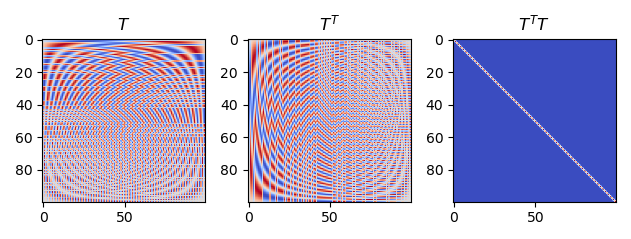
\includegraphics[width=14cm]{p1_2.png}
\caption{}
\end{figure}

\begin{figure}
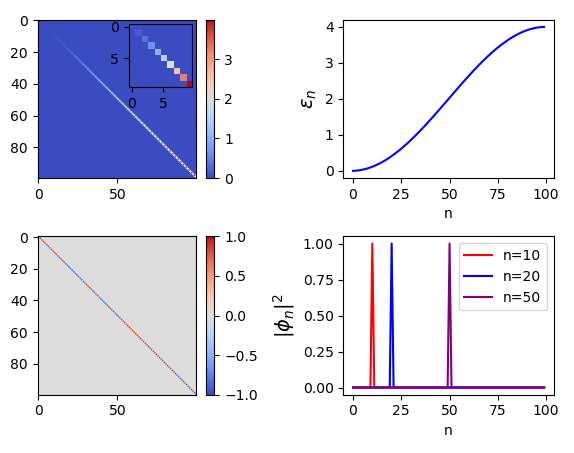
\includegraphics[width=15cm]{p1_3.png}
\caption{}
\end{figure}


These are the solutions to a free particle. The analytical eigenvalues of that problem should be 



\subsection{Source Code}

\begin{lstlisting}[language=Python]
import numpy as np
    
def incmatrix(genl1,genl2):
    m = len(genl1)
    n = len(genl2)
    M = None #to become the incidence matrix
    VT = np.zeros((n*m,1), int)  #dummy variable
    
    #compute the bitwise xor matrix
    M1 = bitxormatrix(genl1)
    M2 = np.triu(bitxormatrix(genl2),1) 

    for i in range(m-1):
        for j in range(i+1, m):
            [r,c] = np.where(M2 == M1[i,j])
            for k in range(len(r)):
                VT[(i)*n + r[k]] = 1;
                VT[(i)*n + c[k]] = 1;
                VT[(j)*n + r[k]] = 1;
                VT[(j)*n + c[k]] = 1;
                
                if M is None:
                    M = np.copy(VT)
                else:
                    M = np.concatenate((M, VT), 1)
                
                VT = np.zeros((n*m,1), int)
    
    return M
\end{lstlisting}

\section{Part II}


\end{document}